\documentclass[14pt,a4paper]{article}
\usepackage{mathtools}
\usepackage{amsmath}
\usepackage{amsthm}
\setcounter{MaxMatrixCols}{20}
\usepackage{mathrsfs}
\usepackage{setspace}
\usepackage{amsfonts}
\usepackage{geometry}
\geometry{a4paper, total = {210mm,297mm},left=25mm, right=20mm,top=25mm,bottom=25mm}
\usepackage{xcolor}
\usepackage{mcode}
\usepackage{listings}
\lstset{basicstyle = \fontsize{11}{12} \selectfont\ttfamily}
\usepackage{graphicx}


%Begin document - Numerical Analysis - Homework 4

\begin{document}
\label{cover}
\begin{center}
	\vspace*{3cm}
	\large{\textbf{MATH/CS 5466 NUMERICAL ANALYSIS \\ Homework 4}}
	\vfill
	\textbf{Luan Cong Doan} \\ luandoan@vt.edu
	%\vfill
%	Department of Mechanical Engineering \\ Virginia Polytechnic Institute and State University
	\vfill
	\today
\end{center}
\pagebreak

\label{Answer Sheet - Numerical Homework 4}
\doublespacing

\label{Problem 1}
\large\textbf{Problem 1.} Clenshaw-Curtis quadrature approximates the integral of a function by the integral of the degree-N polynomial that interpolates it at $N+1$ Chebyshev points: $x_j = \cos(j\pi/N), j = 0, ..., N$. \\
A \texttt{MATLAB} routine for computing the nodes and weights of this rule for the interval $[a,b] = [-1,1]$, called \texttt{clencurt.m} is linked from the course website.
\begin{enumerate}
	\label{1a}
	\item Use Clenshaw-Curtis quadrature (with nodes and weights from \texttt{clencurt.m} to approximate $\int_{-1}^{1}f(x)\mathrm{d}x$ for each of: \\
	\hspace*{2cm} $ f(x) = e^{-x^2}$; \hspace{1.5cm} $f(x) = (1+25x^2)^{-1}$; \hspace{1.5cm} $ f(x) = |x|$ \\
	In particular, for each $f$, produce a \texttt{semilogy} plot showing the degree of interpolating polynomial $N$ versus the error between the Clenshaw-Curtis approximation and the true integral (whose values can be computed in \texttt{MATLAB} via \texttt{sqrt(pi)*erf(1), 2*atan(5)/5} and 1), for $N = 1, ..., 50$ 
	\begin{lstlisting}
	%% 4.1a Clenshaw-Curtis quadrature
	int1 = sqrt(pi)*erf(1);
	int2 = 2*atan(5)/5;
	int3 = 1;
	N = 1:1:50;
	int_approx1 = zeros(1,length(N));
	int_approx2 = zeros(1,length(N));
	int_approx3 = zeros(1,length(N));
	error1 = zeros(1,length(N));
	error2 = zeros(1,length(N));
	error3 = zeros(1,length(N));
	
	for N=1:length(N)
		[x,w] = clencurt(N);
		for j = 1:length(x)
			int_approx1(N) = int_approx1(N) + exp(-x(j).^2)*w(j);
			int_approx2(N) = int_approx2(N) + 1/(1+25*x(j).^2)*w(j);
			int_approx3(N) = int_approx3(N) + abs(x(j))*w(j);
		end
		error1(N) = abs(int_approx1(N) - int1);
		error2(N) = abs(int_approx2(N) - int2);
		error3(N) = abs(int_approx3(N) - int3);
	end
	figure; semilogy(error1); grid on;
	xlabel('N'); ylabel('error'); 
	title('Clenshaw-Curtis approximation error of exp(-x^2)');
	print('hw4_1a1','-dpng');
	figure; semilogy(error2); grid on;
	xlabel('N'); ylabel('error'); 
	title('Clenshaw-Curtis approximation error of (1+25*x^2)^(-1)');
	print('hw4_1a2','-dpng');
	figure; semilogy(error3); grid on;
	xlabel('N'); ylabel('error'); 
	title('Clenshaw-Curtis approximation error of |x|');
	print('hw4_1a3','-dpng');
	\end{lstlisting}
	\begin{figure}[htp]
		\centering
		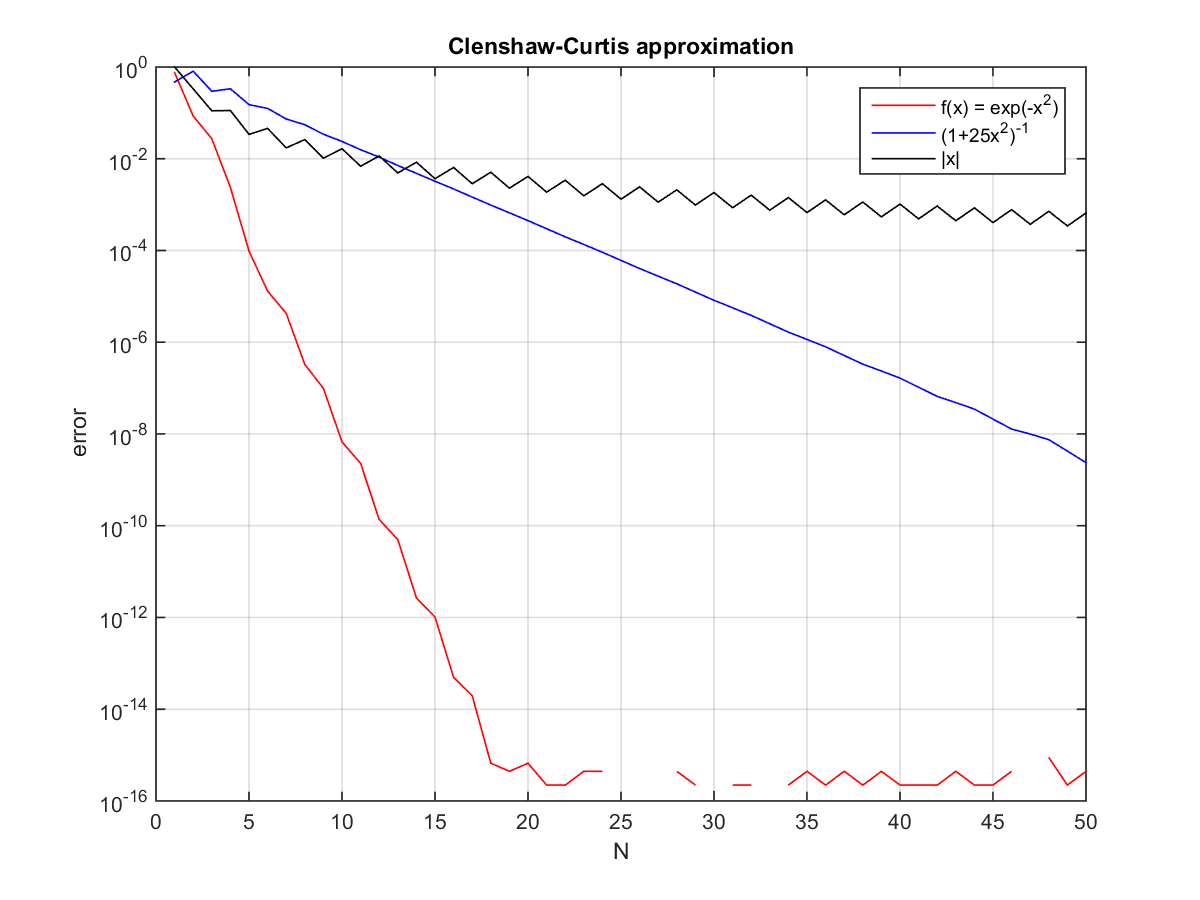
\includegraphics[scale=0.7]{hw4_1a.png}
		\caption{Clenshaw-Curtis aprroximation error of $f(x)=e^{-x^2}, (1+25x^2)^{-1}, |x|$}
	\end{figure}
	\pagebreak
%	\begin{figure}[htp]
%		\centering
%		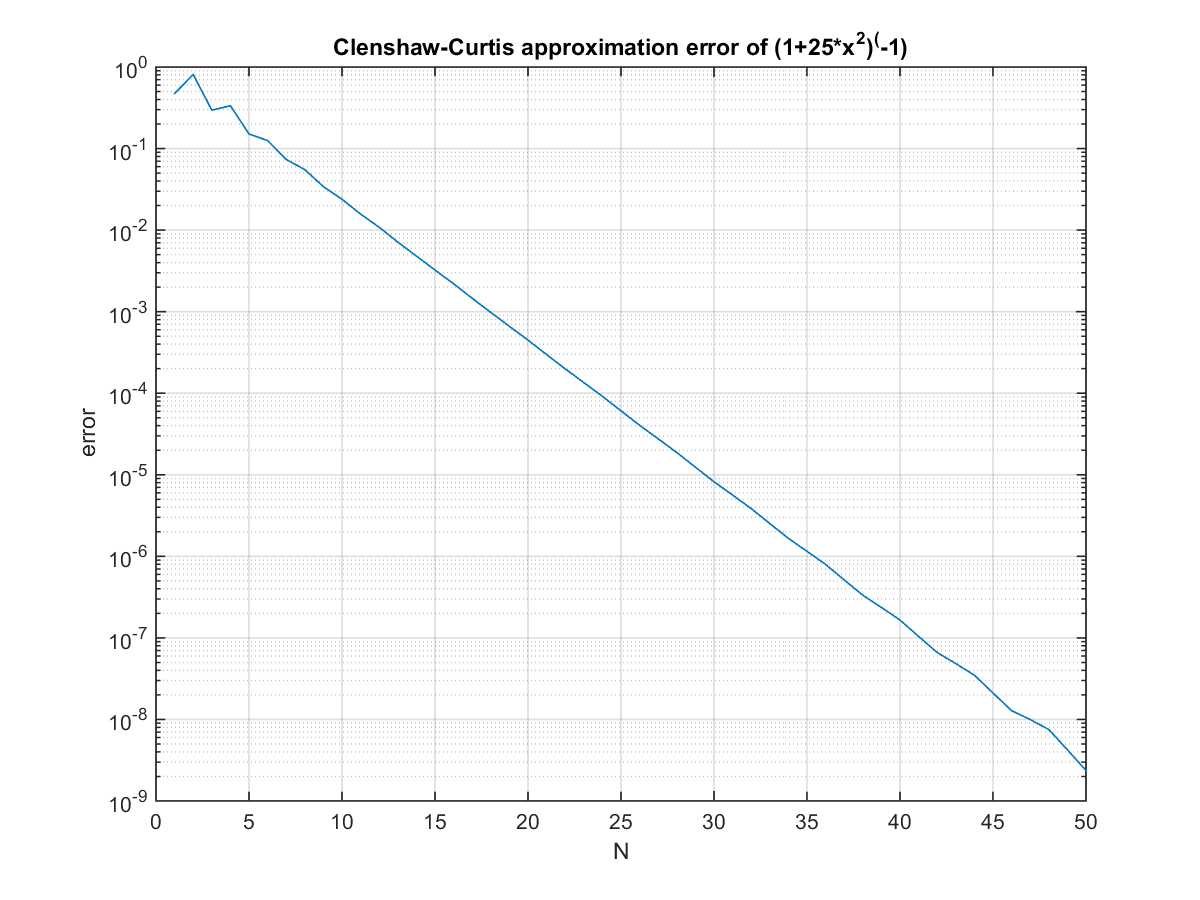
\includegraphics[scale=0.55]{hw4_1a2.png}
%		\caption{Clenshaw-Curtis aprroximation error of $f(x)=(1+25x^2)^{-1}$}
%	\end{figure}
%	\begin{figure}[htp]
%		\centering
%		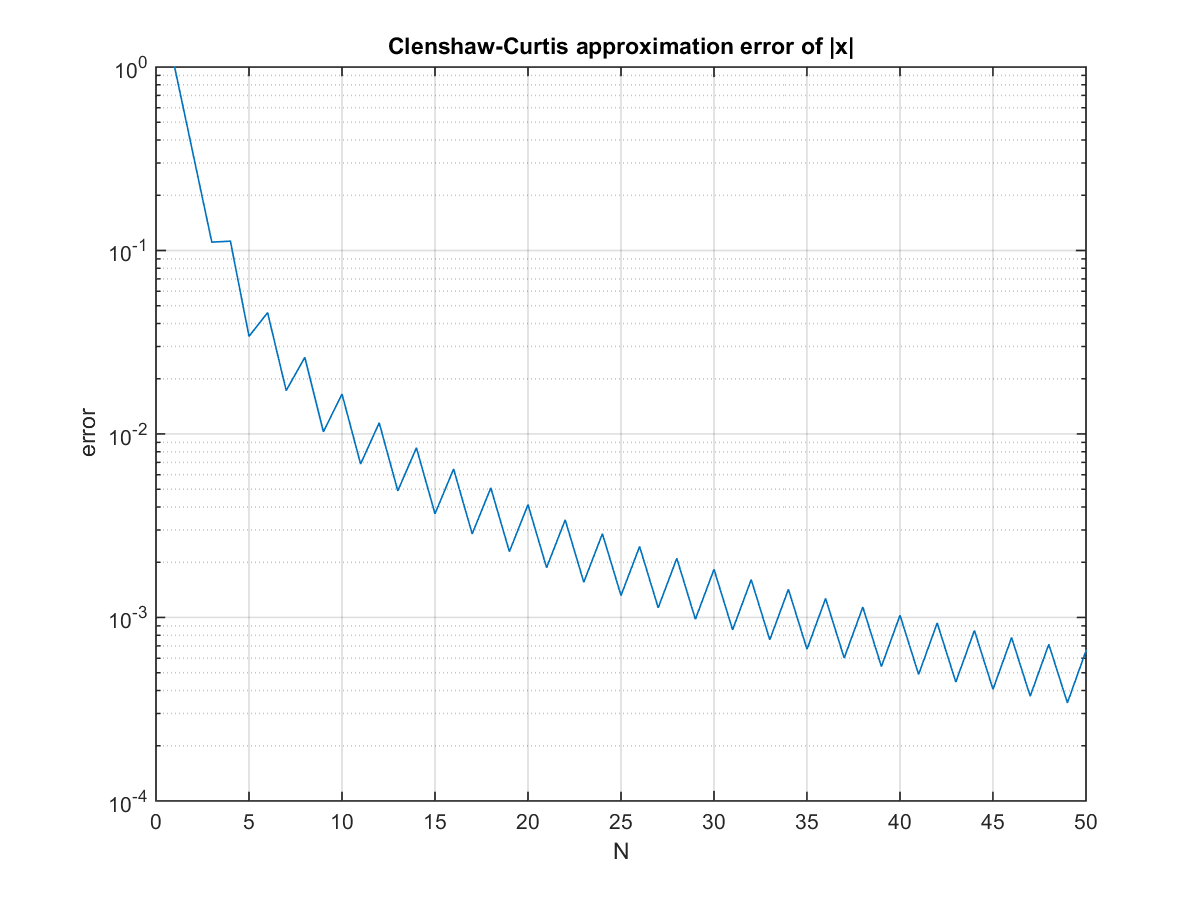
\includegraphics[scale=0.55]{hw4_1a3.png}
%		\caption{Clenshaw-Curtis aprroximation error of $f(x)=|x|$}
%	\end{figure}
	
	\label{1b}
	\item Why do you think the three different function in part (a) produce such different results? \\
	The integral of the first function $f = e^{-x_i^2}$ is most close to the function itself, (e.g. $(e^x)' = e^x$), and the last function is further different from original f. That lead to the Clenshaw-Curtis approximation is different in accuracy.\\
	%For the same value of $x_i$ value of these 3 function increasing: $ e^{-x_i^2} < (1+20x^2)^{-1} < |x|$ so the error of them should be in the same order (because they have the same weight $w_i$)\\
	
	
	\label{1c}
	\item For the first function, $f(x) = e^{-x^2}$, use \texttt{MATLAB}'s \texttt{tic} and \texttt{toc} commands to time how long it takes compute the Clenshar-Curtis approximation for $N = 20$ (include the time for computing the nodes and weights). Compare this value to the time required to integrate this same $f$ using \texttt{MATLAB}'s all-purpose adaptive quadrature routine, \texttt{quad}, with precision \texttt{1e-15}. 
	\begin{lstlisting}
	%% tic and toc utilize clencurt
	tic
	int_approx = 0;
	[x,w] = clencurt(20);
	for j = 1:length(x)
		int_approx = int_approx + exp(-x(j).^2)*w(j);
	end
	toc
	Elapsed time is 0.001829 seconds.
	%% tic toc quad function
	tic
	f = @(x) exp(-x.^2);
	q = quad(f,-1,1);
	toc
	Elapsed time is 0.003241 seconds.
	\end{lstlisting}
	For N = 20, the first approach using Clenshaw-Curtis approximation is about $150\%$ faster than compute integral directly by utilizing \texttt{MATLAB's quad} function.
	
\end{enumerate}
\pagebreak

\label{Problem 2}
\large\textbf{Problem 2.} You may use the following facts without proof: For the positive integers $N$ and $n$ 
$$ \sum_{k=1}^{N}\sin\left(\dfrac{2\pi nk}{N} \right) = 0 \hspace{1cm} and \hspace{1cm} \sum_{k=1}^{N}\cos\left(\dfrac{2\pi nk}{N}\right) = \begin{cases} N \quad if \hspace{2mm} n/N \hspace{1mm} is\hspace{1mm} an \hspace{1mm} integer \\ 0 \quad otherwise \end{cases} $$
 
\begin{enumerate}
	\label{2a} 
	\item Write down the composite trapezoid rule for approximating:
	$$ \int_{a}^{b} f(x)\mathrm{d}x $$
	with function evaluation at $x_k = a + kh$ for $ h = (b-a)/N$ and $ k = 0, ..., N$
	\begin{align*} \int_{a}^{b} f(x)\mathrm{d}x  &= \sum_{k=1}^{N}\int_{x_{k-1}}^{x_k} f(x)\mathrm{d}x \approx \sum_{k=1}^{N} \dfrac{x_k - x_{k-1}}{2} [f(x_{k-1}) + f(x_k)] \\
	&= \dfrac{h}{2} \left[ \sum_{k=1}^{N}f(x_{k-1}) + \sum_{k=1}^{N} f(x_k) \right] \\
	&= \dfrac{h}{2} \left[ f(x_0) + 2\sum_{k=1}^{N-1}f(x_k) + f(x_N) \right] \end{align*}
		
	\label{2b}	
	\item Suppose we wish to approximate
	$$ \int_{0}^{2\pi} f(x)\mathrm{d}x$$
	where $f$ is a $2\pi$-periodic function (that is, $f(x) = f(x + 2\pi)$ for all $x \in \mathbb{R}$ \\
	Applied above result we have: $f(x_0) = f(0); f(x_N) = f(2\pi)$ and $f(0) = f(2\pi)$:
	\begin{align*} \int_{0}^{2\pi} f(x)\mathrm{d}x  = \dfrac{h}{2} \left[ f(x_0) + 2\sum_{k=1}^{N-1}f(x_k) + f(x_N) \right]  &= \dfrac{h}{2} \left[ f(0) + 2\sum_{k=1}^{N-1}f(x_k) + f(0 + 2\pi) \right] \\
	%$$ \Leftrightarrow \int_{0}^{2\pi} f(x)\mathrm{d}x  
	&= \dfrac{h}{2} \left[ 2\sum_{k=1}^{N-1}f(x_k) + 2f(x_N) \right]\\ &= \dfrac{h}{2}* 2\sum_{k=1}^{N}f(x_k) \\ &= h\sum_{k=1}^{N}f(x_k)\end{align*}
	We have: $h = \dfrac{2\pi - 0}{N} = \dfrac{2\pi}{N}$ and $x_k = x_0 + kh = 0 + k\dfrac{2\pi}{N} = \dfrac{2\pi k}{N}$ so:
	$$ \int_{0}^{2\pi} f(x)\mathrm{d}x  = h\sum_{k=1}^{N}f(x_k) = \dfrac{2\pi}{N} \sum_{k=1}^{N} f\left(\dfrac{2\pi k}{N}\right) $$
	
		\textbf{\textit{For the rest of the problem}}: suppose $f$ is a $2\pi$-periodic function with Fourier series
	$$ f(x) = \dfrac{c_0}{\sqrt{2\pi}} + \sum_{n=1}^{\infty} c_{-n} \dfrac{1}{\sqrt{\pi}}\cos(nx) + \sum_{n=1}^{\infty} c_n \dfrac{1}{\sqrt{\pi}}\sin(nx)$$
	for constants $c_0, c_1, ... $
	\label{2c}
	\item Integrate each term of this Fourier series to obtain a simple formula for $\int_{0}^{2\pi} f(x)\mathrm{d}x$ \\
	Because $f$ is a $2\pi$-periodic function, so applied result from (2b) we have:
	%\begin{equation}
	\begin{align*} \int_{0}^{2\pi} f(x)\mathrm{d}x  &= \dfrac{2\pi}{N} \sum_{k=1}^{N} f\left(\dfrac{2\pi k}{N}\right) \\ 
	&= \dfrac{2\pi}{N} \sum_{k=1}^{N} \left( \dfrac{c_0}{\sqrt{2\pi}} + \sum_{n=1}^{\infty} c_{-n} \dfrac{1}{\sqrt{\pi}}\cos(n\dfrac{2\pi k}{N}) + \sum_{n=1}^{\infty} c_n \dfrac{1}{\sqrt{\pi}}\sin(n\dfrac{2\pi k}{N}) \right) \\
	&= \dfrac{2\pi}{N}\sum_{k=1}^{N}\dfrac{c_0}{\sqrt{2\pi}} + \dfrac{2\pi}{N\sqrt{\pi}} \sum_{n=1}^{\infty} \left(\sum_{k=1}^{N}c_{-n}\cos\left(\dfrac{2\pi nk}{N}\right) + \sum_{k=1}^{N}c_n\sin\left(\dfrac{2\pi nk}{N}\right) \right) \\
	&= c_0\sqrt{2\pi} + \dfrac{2\sqrt{\pi}}{N}\sum_{n=1}^{\infty} \left(c_{-n}\sum_{k=1}^{N}\cos\left(\dfrac{2\pi nk}{N}\right) + c_n\sum_{k=1}^{N}\sin\left(\dfrac{2\pi nk}{N}\right) \right) \end{align*}
	
	Utilize the given condition, we have:
	%+ If $n/N$ is not an integer:
	%$$ \int_{0}^{2\pi} f(x)\mathrm{d}x = c_0\sqrt{2\pi}$$
	%+ If $n/N$ is an integer:
	$$ \int_{0}^{2\pi} f(x)\mathrm{d}x = c_0\sqrt{2\pi} + \dfrac{2\sqrt{\pi}}{N}\sum_{n=kN}^{\infty}c_{-n}N = c_0\sqrt{2\pi} + 2\sqrt{\pi} \sum_{n=kN}^{\infty}c_{-n} \hspace{0.5cm} for \hspace{0.2cm} k = 1,2,...$$ %= 2\sqrt{\pi} \sum_{n=0}^{\infty}c_{-n}$$
		
	\label{2d}
	\item Write down a descriptive bound for the difference between the true integral found in part (c) and the approximation obtained from the composite trapezoid rule applied to the function $f$ with the above Fourier series. 
	\begin{align*} \int_{0}^{2\pi} f(x)\mathrm{d}x &= \int_{0}^{2\pi} \left( \dfrac{c_0}{\sqrt{2\pi}} + \sum_{n=1}^{\infty} c_{-n} \dfrac{1}{\sqrt{\pi}}\cos(nx) + \sum_{n=1}^{\infty} c_n \dfrac{1}{\sqrt{\pi}}\sin(nx) \right) \mathrm{d}x \\
	&= \int_{0}^{2\pi} \dfrac{c_0}{\sqrt{2\pi}}\mathrm{d}x \\
	&= c_0\sqrt{2\pi}
	\end{align*}
	The error bound is defined:
	\begin{align*} Error &= \int_{0}^{2\pi} f(x)\mathrm{d}x - c_0\sqrt{2\pi} - 2\sqrt{\pi} \sum_{n=kN}^{\infty}c_{-n} \\
	&= c_0\sqrt{2\pi} - c_0\sqrt{2\pi} - 2\sqrt{\pi} \sum_{n=kN}^{\infty}c_{-n} \\
	&= - 2\sqrt{\pi} \sum_{n=kN}^{\infty}c_{-n} \hspace{1.5cm} for \hspace{0.2cm} k = 1,2,... \end{align*}
	
	\label{2e}
	\item If $f$ and its first $p > 1$ derivatives are continuous and $2\pi$-periodic, then there exists a constant $\gamma$ such that $|c_{|n|}| \leq \gamma/|n|^p$ for all integers $n$. Compare the performance of the composite trapezoid rule applied to such an $f$ with the usual composite trapezoid error bound that holds for functions that are in $C^2$, but not necessary  $2\pi$-periodic.
	$$ f^{(1)} = -\sum_{n=1}^{\infty} n.c_{-n} \dfrac{1}{\sqrt{\pi}}\sin(nx) + \sum_{n=1}^{\infty} n.c_n \dfrac{1}{\sqrt{\pi}}\cos(nx)$$
	\begin{align*} f^{(2)} &= -\sum_{n=1}^{\infty} n^2.c_{-n} \dfrac{1}{\sqrt{\pi}}\cos(nx) - \sum_{n=1}^{\infty} n^2.c_n \dfrac{1}{\sqrt{\pi}}\sin(nx) \\
	&= \sum_{n=1}^{\infty} \dfrac{n^2}{\sqrt{\pi}} \left(-c_{-n}\cos(nx) - c_n\sin(nx)\right)\\
	&\leq \sum_{n=1}^{\infty} \dfrac{\gamma}{\sqrt{\pi}} \left(\cos(nx) + \sin(nx)\right)  \end{align*}
	$$ \int_{0}^{2\pi} f(x)\mathrm{d}x - \int_{0}^{2\pi} p(x)\mathrm{d}x =  -\dfrac{1}{12}f^{(2)}(\eta)(2\pi-0)^3 %\hspace{1cm} \eta \in [0,2\pi] \\
	\geq -\dfrac{8\pi^3}{12}\sum_{n=1}^{\infty} \dfrac{\gamma}{\sqrt{\pi}} \left(\cos(n\eta) + \sin(n\eta)\right)  
%	&\geq -\dfrac{8\pi^3}{12}\sum_{n=1}^{\infty} \dfrac{\gamma}{\sqrt{\pi}} \sqrt{2}
	$$ %end{align*}$$
	
	\label{2f} 
	\item Produce a \texttt{loglog} plot comparing the error in the trapezoid rule approximation to the $2\pi$-periodic problem:
	$$ \int_{0}^{2\pi} \exp(\sin(x))\mathrm{d}x = 7.95492652101284527451322...$$	
		and the smooth but bot $2\pi$-periodic problem:
	$$ \int_{0}^{2\pi} \exp(\sin(x/\pi))\mathrm{d}x = 13.3094551602297896414536...$$
	%\pagebreak
	\begin{lstlisting}
	fx1 = @(x) exp(sin(x));
	fx2 = @(x) exp(sin(x/pi));
	it1 = 7.9549265210128452745132;
	it2 = 13.3094551602297896414536;
	for i =1:5 %length(N)
		N = 10^(i);
		Ifx1(i) = trapezoid(fx1,0,2*pi,N);
	end
	errorF1 = abs(Ifx1 - it1);
	
	for i =1:5 %length(N)
		N = 10^(i);
		Ifx2(i) = trapezoid(fx2,0,2*pi,N);
	end
	errorF2 = abs(Ifx2 - it2);
	figure; loglog(errorF1,'r'); hold on;
	loglog(errorF2,'b--'); grid on;
	xlabel('N'); ylabel('error');
title('loglog plot of error in trapezoid approximation of exp(sin(x))');
	legend('Error 1','Error 2');
	print('hw4_2f','-dpng');
	\end{lstlisting}
	\begin{figure}[htp]
		\centering
		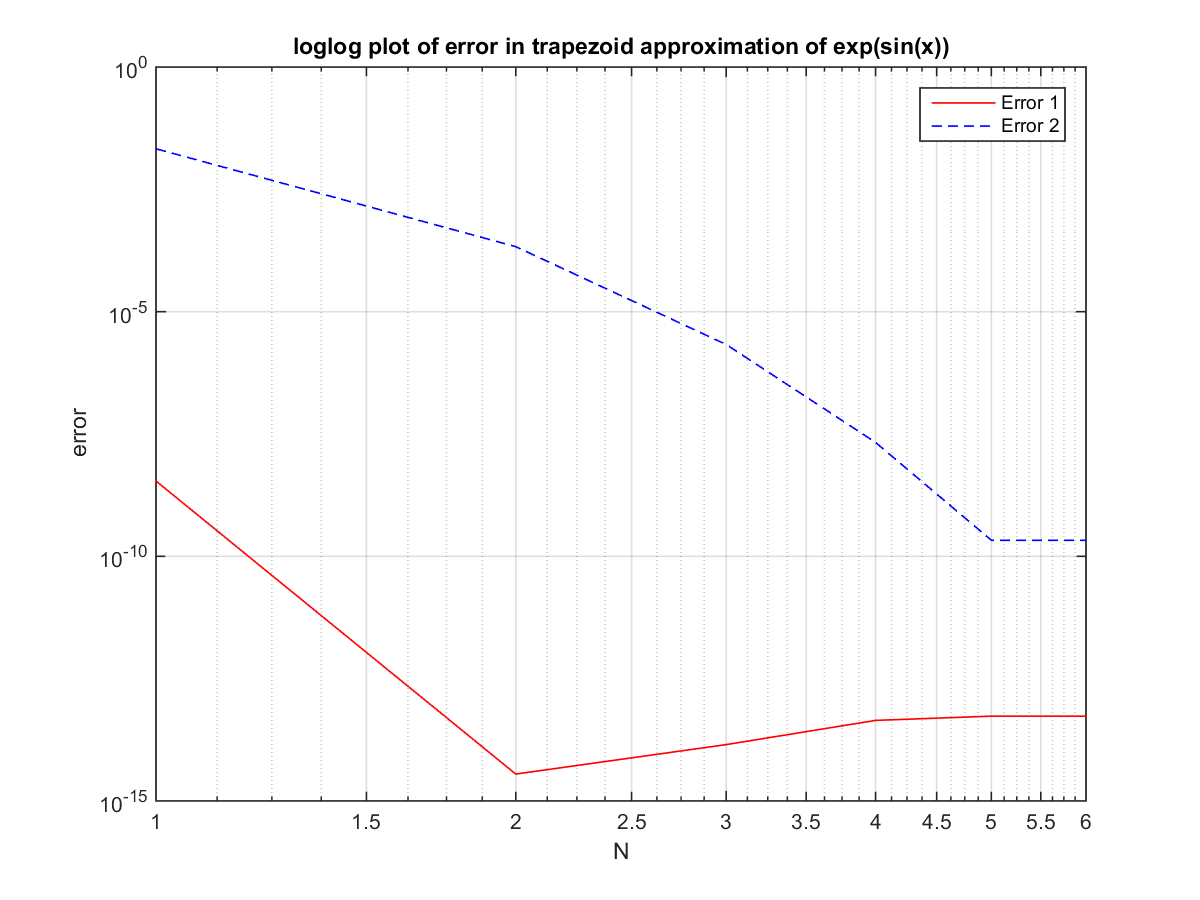
\includegraphics[scale=0.5]{hw4_2f.png}
		\caption{Comparing the error in the trapezoid rule approximation}
	\end{figure} 
%	For a different approach (check):
%	\begin{lstlisting}
%	fx1 = @(x) exp(sin(x));
%	fx2 = @(x) exp(sin(x/pi));
%	it1 = 7.9549265210128452745132;
%	it2 = 13.3094551602297896414536;
%	Ifx1 = zeros(1,length(N));
%	Ifx2 = zeros(1,length(N));
%	for i =1:length(N)
%		Ifx1(i) = trapezoid(fx1,0,2*pi,i);
%		Ifx2(i) = trapezoid(fx2,0,2*pi,i);
%	end
%	errorF1 = abs(Ifx1 - it1) ;
%	figure; loglog(errorF1); grid on;
%	xlabel('N'); ylabel('error');
%	title('loglog plot of error in trapezoid approximation of exp(sin(x))');
%	print('hw4_2f1','-dpng');
		
%	errorF2 = Ifx2 - it2;
%	figure; loglog(errorF2); grid on;
%	xlabel('N'); ylabel('error');
%	title('loglog plot of error in trapezoid approximation of exp(sin(x/pi))');
%	print('hw4_2f2','-dpng');
%	\end{lstlisting}
%	\begin{figure}[htp]
%		\centering
%		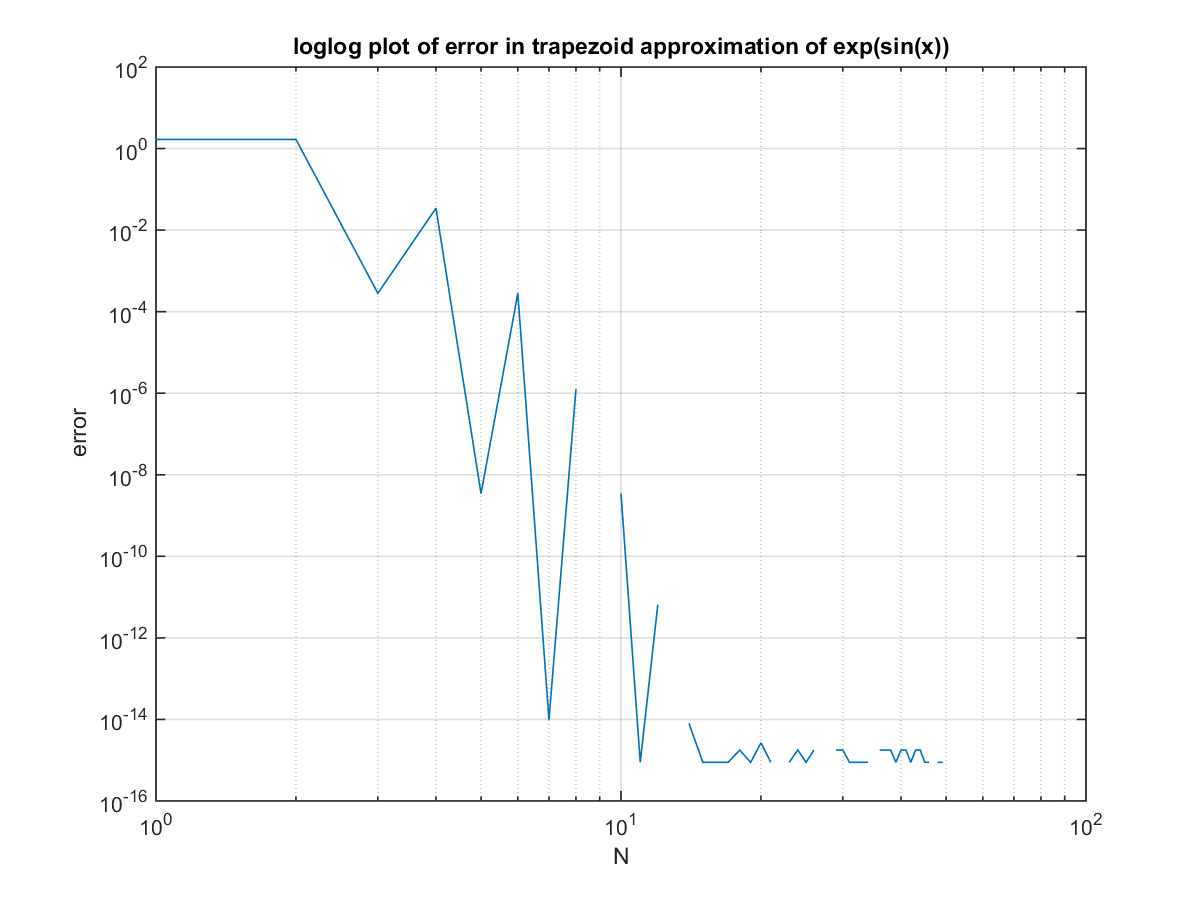
\includegraphics[scale=0.75]{hw4_2f1.png}
%		\caption{Comparing the error in the trapezoid rule approximation to the $%2\pi$-periodic}
%	\end{figure} 
%	\begin{figure}[htp]
%		\centering
%		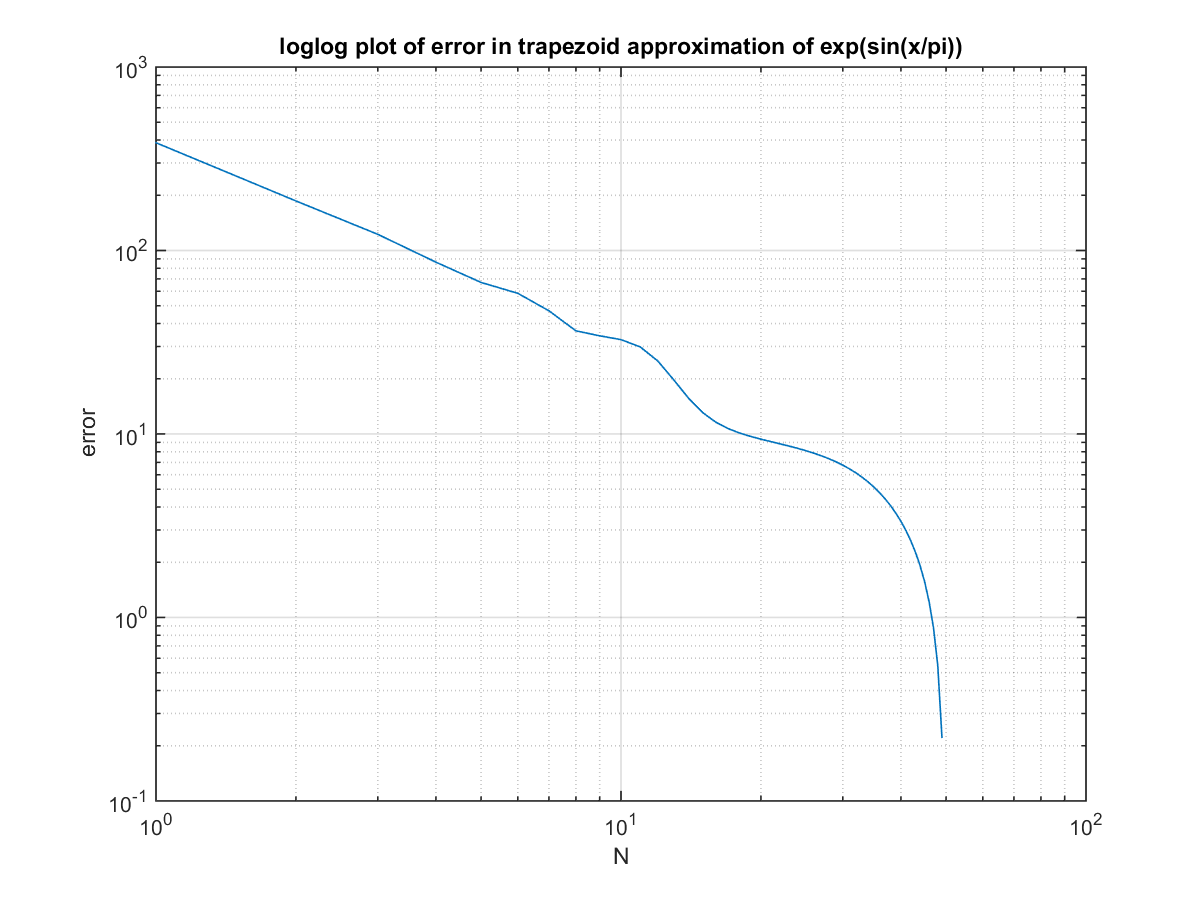
\includegraphics[scale=0.75]{hw4_2f2.png}
%		\caption{Comparing the error in the trapezoid rule approximation to the not $%2\pi$-periodic}
%	\end{figure} 
\end{enumerate}

\label{Problem 3}
\large\textbf{Problem 3.} Let $\langle f,g\rangle$ denote a weighted inner product on $L^2(a,b)$, e.g, $\langle f,g\rangle = \int_{a}^{b}f(x)g(x)w(x)\mathrm{d}x$ for some appropriate weight function $w$: 

\begin{enumerate}
	\label{3a}
	\item Suppose $\{\phi_j\}_{j=0}^n$ is a system for \textit{monic} orthogonal polynomials, and let:
	$$ \phi_{n+1}(x) = x\phi_n(x) - \sum_{j=0}^{n} c_{n,j}\phi_j(x) \hspace{1cm} (*)  $$
	denote the next polynomial in this system. For $n \geq 1$, show that we can write\\
	$ \phi_{n+1}(x) = x\phi_n(x) - \alpha_n\phi_n(x) - \beta_n\phi_{n-1}(x)$ \\
	where $\alpha_n$ and  $\beta_n$ are constants that you should specify. (This was worked out in the lectures, but the result is sufficiently important that you should work through the details for yourself).\\
	$\{\phi_j\}_{j=0}^n$ is a system for \textit{monic} orthogonal polynomials, so: $\phi_{-1} = 0; \phi_0 = 1$
	$$ \phi_{n+1}(x) - x\phi_n(x) = - \sum_{j=0}^{n} c_{n,j}\phi_j(x) \hspace{1cm} (*) $$
	Applied orthogonality properties: inner product with $\phi_k(x)$ with $k \leq n$
	\begin{align*} \langle \phi_{n+1}(x) - x\phi_n(x), \phi_k(x) \rangle &= - \sum_{j=0}^{n} \langle c_{n,j}\phi_j(x), \phi_k(x) \rangle \\ 
	\Leftrightarrow \langle \phi_{n+1}(x), \phi_k(x)\rangle - \langle x\phi_n(x), \phi_k(x) \rangle &= - \sum_{j=0}^{n} c_{n,j} \langle \phi_j(x), \phi_k(x) \rangle \\
	\Leftrightarrow -\langle x\phi_n(x), \phi_k(x) \rangle &= -c_{n,k}\langle \phi_k(x), \phi_k(x) \rangle \\
	\Leftrightarrow \langle \phi_n(x), x \phi_k(x) \rangle &= c_{n,k}\langle \phi_k(x), \phi_k(x) \rangle \hspace{1cm} (**) \end{align*} 
	If $ k < n-1 \Rightarrow \mathrm{deg}(x\phi_k(x)) < n \Rightarrow \langle \phi_n(x), x \phi_k(x) \rangle = 0 \Rightarrow c_{n,k} = 0$ \\
	Applied above result to provided equation (*):\\
	\hspace*{2cm} $ \phi_{n+1}(x) = x\phi_n(x) + c_{n,n-1}\phi_{n-1}(x) + c_{n,n}\phi_n(x) $ for $n = 1,2,3,  ...$\\
	From (**) we have: $ \alpha_n = c_{n,n} = \left.\dfrac{\langle \phi_n(x), x \phi_k(x) \rangle}{\langle \phi_k(x), \phi_k(x) \rangle} \right|_{k=n} = \dfrac{\langle \phi_n(x), x \phi_n(x) \rangle}{\langle \phi_n(x), \phi_n(x) \rangle} $ \\
	 and $ \beta_n = c_{n,n-1} = \left.\dfrac{\langle \phi_n(x), x \phi_k(x) \rangle}{\langle \phi_k(x), \phi_k(x) \rangle}\right|_{k=n-1} = \dfrac{\langle \phi_n(x), x \phi_{n-1}(x) \rangle}{\langle \phi_{n-1}(x), \phi_{n-1}(x) \rangle} = \dfrac{\langle \phi_n(x), \phi_n(x) \rangle}{\langle \phi_{n-1}(x), \phi_{n-1}(x) \rangle} $
	So, we can rewrite (*) as: \\
	\hspace*{3cm} $ \phi_{n+1}(x) = x\phi_n(x) - \alpha_n\phi_n(x) - \beta_n\phi_{n-1}(x)$ 
	
	\label{3b}
	\item Consider the \textit{Jacobi} matrix and vector \\
	\hspace*{1cm} $ \textbf{J} = \begin{bmatrix} \alpha_0 & \sqrt{\beta_1} & ... & ... & ... \\ \sqrt{\beta_1} & \alpha_1 & \sqrt{\beta_2} & ... & ... \\ ... & \sqrt{\beta_2} & \ddots & \ddots \\ ... & ... & \ddots & \alpha_{n-1} & \sqrt{\beta_n} \\ ... & ... & ... & \sqrt{\beta_n} & \alpha_n \end{bmatrix},  \hspace{1cm} \textbf{v}(x) = \begin{bmatrix} \phi_0(x) \\ \phi_1(x)/\sqrt{\beta_1} \\ \phi_2(x)/\sqrt{\beta_1\beta_2} \\ ... \\ \phi_n(x)/\sqrt{\beta_1...\beta_n} \end{bmatrix}$ \\
	(For $n \geq 1$, $\alpha_n$ and $\beta_n$ are as in part (a); $\alpha_0$ is defined by $\phi_1(x) = x\phi_0(x) - \alpha_0\phi_0(x)$ \\
	Verify that $(\lambda,v(\lambda))$ is an eigenpair of \textbf{J} if and only if $\lambda$ is a root of $\phi_{n+1}$ \\ 
	With $\lambda$ is a eigenvalue of \textbf{J} we have: $\mathrm{det}[\textbf{J} - \lambda\textbf{I}] =0$\\
	Assume that $(\lambda,v(\lambda))$ is an eigenpair of \textbf{J} so: $\textbf{J}v(\lambda) = \lambda v(\lambda)$\\ 
	We first have:
	\begin{align*} \textbf{J}v(\lambda) - \lambda v(\lambda) &= \begin{bmatrix} \alpha_0 & \sqrt{\beta_1} & ... & ... & ... \\ \sqrt{\beta_1} & \alpha_1 & \sqrt{\beta_2} & ... & ... \\ ... & \sqrt{\beta_2} & \ddots & \ddots \\ ... & ... & \ddots & \alpha_{n-1} & \sqrt{\beta_n} \\ ... & ... & ... & \sqrt{\beta_n} & \alpha_n \end{bmatrix}.\begin{bmatrix} \phi_0(\lambda) \\ \phi_1(\lambda)/\sqrt{\beta_1} \\ \phi_2(\lambda)/\sqrt{\beta_1\beta_2} \\ ... \\ \phi_n(\lambda)/\sqrt{\beta_1...\beta_n} \end{bmatrix} - \lambda\begin{bmatrix} \phi_0(\lambda) \\ \phi_1(\lambda)/\sqrt{\beta_1} \\ \phi_2(\lambda)/\sqrt{\beta_1\beta_2} \\ ... \\ \phi_n(\lambda)/\sqrt{\beta_1...\beta_n} \end{bmatrix}\\
	&= \begin{bmatrix} \alpha_0\phi_0(\lambda) + \phi_1(\lambda) - \lambda. \phi_0(\lambda)\\ \sqrt{\beta_1}\phi_0(\lambda) + \alpha_1\phi_1(\lambda)/\sqrt{\beta_1} + \sqrt{\beta_2}\phi_2(\lambda)/\sqrt{\beta_1\beta_2} - \lambda\phi_1(\lambda)/\sqrt{\beta_1} \\ \sqrt{\beta_2}\phi_1(\lambda)/\sqrt{\beta_1} + \alpha_2\phi_2(\lambda)/\sqrt{\beta_1\beta_2} + \sqrt{\beta_3}\phi_3(\lambda)/\sqrt{\beta_1\beta_2\beta_3} - \lambda\phi_2(\lambda)/\sqrt{\beta_1\beta_2} \\ ... \\ \sqrt{\beta_n}\phi_{n-1}/\sqrt{\beta_1\beta_2...\beta_{n-1}} + \alpha_n\phi_n(\lambda)/\sqrt{\beta_1...\beta_n} - \lambda \phi_n(\lambda)/\sqrt{\beta_1...\beta_n} \end{bmatrix} \\
	&= \begin{bmatrix} \alpha_0\phi_0(\lambda) + \phi_1(\lambda) - \lambda\phi_0(\lambda) \\ \dfrac{1}{\sqrt{\beta_1}}\left( \beta_1\phi_0 + \alpha_1\phi_1(\lambda) + \phi_2(\lambda) - \lambda\phi_1(\lambda) \right) \\ \dfrac{1}{\sqrt{\beta_1\beta_2}}\left( \beta_2\phi_1 + \alpha_2\phi_2(\lambda) + \phi_3(\lambda) - \lambda\phi_2(\lambda) \right) \\ \cdots \\ \dfrac{1}{\sqrt{\beta_1\cdots\beta_n}}\left( \beta_n\phi_{n-1} + \alpha_n\phi_n(\lambda) - \lambda\phi_n(\lambda) \right)\end{bmatrix} \hspace{2cm} (***)\end{align*}
	
	We have that $\textbf{J}v(\lambda) = \lambda v(\lambda) \Leftrightarrow \textbf{J}v(\lambda) - \lambda v(\lambda) = 0$	\\
	With respect to $\alpha_n, \beta_n$ from part (3a) $\Rightarrow (\lambda, v(\lambda))$ is a eigenpair if and only if  (***) is true $\Rightarrow \lambda$ is a root of $\phi_j$ with $ j = 0,1, ... , n$\\
	As a result: $ \phi_{n+1} = x\phi_n(x) - \alpha_n\phi_n(x) - \beta_n\phi{n-1}(x) \\
	\hspace*{1.6cm} \Rightarrow \phi_{n+1}(\lambda) = \lambda\phi_n(\lambda) - \alpha_n\phi_n(\lambda) - \beta_n\phi{n-1}(\lambda) \\
	\hspace*{3.7cm} = \lambda.0 - \alpha_n.0 - \beta_n.0 \\ \hspace*{3.7cm} = 0 $\\
	$\Rightarrow \lambda$ is a root of $\phi_{n+1}$
\end{enumerate}

\label{Problem 4}
\large\textbf{Problem 4.} \textit{Monte Carlo methods} provide an alternative to interpolatory quadrature schemes. Given $f \in C[a,b]$, from a probabilistic perspective one can interpret the integral of $f$ as its \textit{expected values}:
$$ \int_{a}^{b} f(x)\mathrm{d}x =: E[f]$$
The expected value $E[f]$ is just another name for the \textit{mean}, which can be estimated by averaging value of $f$ sampled at uniformly distributed random points in $[a,b]$. Hence, the $N$-points \textit{Monte Carlo} estimate of the integral is given by
$$ \int_{a}^{b} f(x)\mathrm{d}x \approx \dfrac{b-a}{N} \sum_{k=1}^{N}f(\xi_j)$$
where $\xi_1, ..., \xi_N$ are $N$ independent samples of a uniform random variable over $[a,b]$, as can be generated using \texttt{MATLAB's rand} command. The Central Limit Theorem suggests that this estimate will converge to the exact integral at a rate of $N^{-1/2}$.

\begin{enumerate}
	\label{4a}
	\item Consider the function $f(x) = \sin(x)$ over $x \in [0,2]$. Produce a \texttt{loglog} plot comparing $N$ versus error for the $N$-point Monte Carlo method and the trapezoid rule based on $N$ function evaluations, for various values of $N$ (Take your largest $N$ to be at least $10^5$.) Which method is superior?
	\begin{lstlisting}
	% Monte Carlo points
	IfM = zeros(1,N);
	for i = 1:N
		xi = rand(1,i)*2;
		for j = 1:i
			IfM(i) = IfM(i) + (2/i)*sin(xi(j));
		end
	end
	errorM = abs(IfM - int);
	% trapezoid rule
	IfT = zeros(1,N);
	for i = 1:N
		IfT(i) = trapezoid(fx,0,2,i);
	end
	errorT = abs(IfT - int);
figure; loglog(errorM); hold on; 
loglog(errorT); grid on;
xlabel('N'); ylabel('error');
title('loglog plot of error from MonteCarlo & Trapezoid for f(x)=sin(x)');
legend('Monte Carlo','Trapezoid');
print('hw4_4a','-dpng');
	\end{lstlisting}
	\begin{figure}[htp]
		\centering
		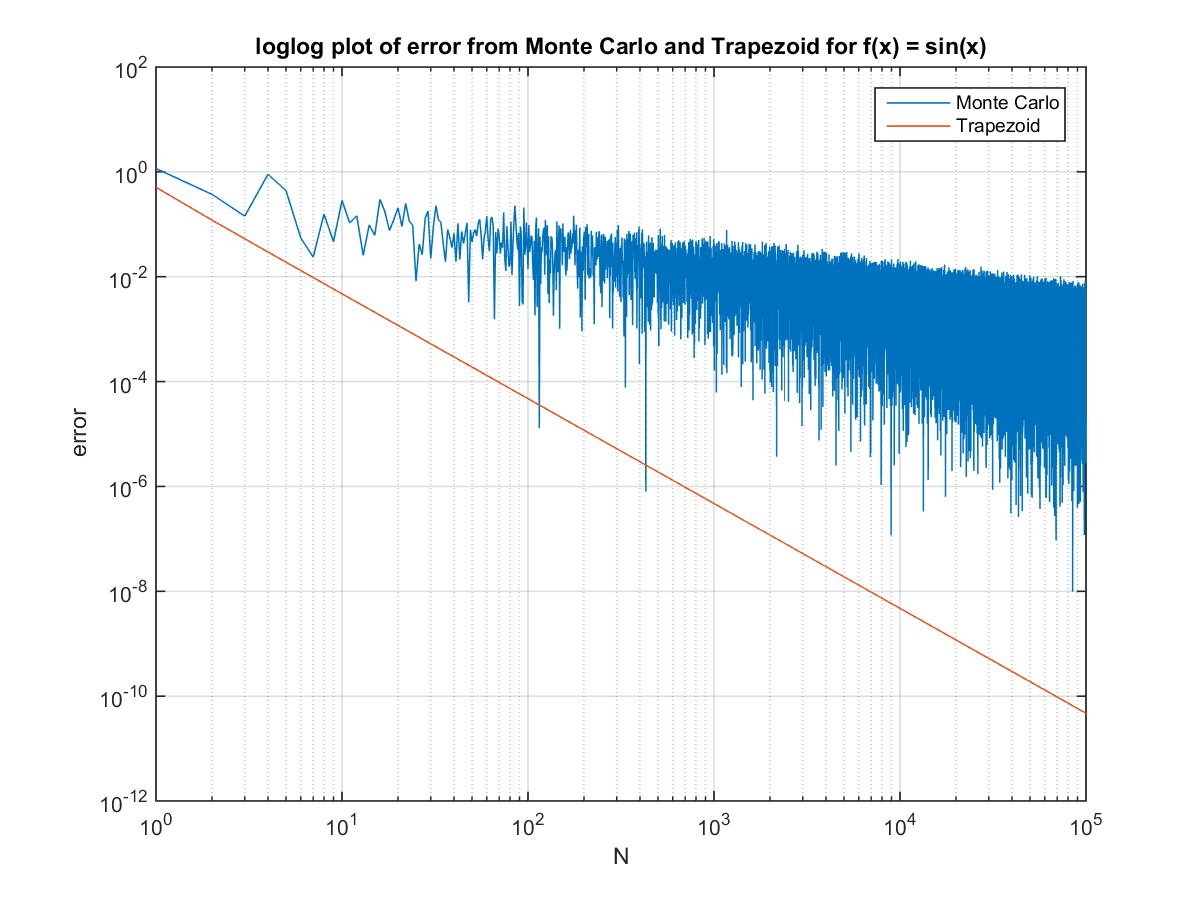
\includegraphics[scale=0.65]{hw4_4a.png}
		\caption{loglog plot of error from MonteCarlo and Trapezoid for $f(x)=\sin(x)$}
	\end{figure}
	We see that for trapezoid rule provide better result, but the computation is more expensive than Monte Carlo method, it requires more time to process (around 1.5 times of Monte Carlo's time). So depend on how much accuracy needed, we can choose the better one.\\
	
	The rest of problem concerns approximation of a 10-dimensional integral:
	$$ \int_{a}^{b} \int_{a}^{b} \int_{a}^{b} \int_{a}^{b} \int_{a}^{b} \int_{a}^{b} \int_{a}^{b} \int_{a}^{b} \int_{a}^{b} \int_{a}^{b} f(x_1,x_2,x_3,x_4,x_5,x_6,x_7,x_8,x_9,x_{10}) \mathrm{d}x_1\mathrm{d}x_2\mathrm{d}x_3\mathrm{d}x_4\mathrm{d}x_5\mathrm{d}x_6\mathrm{d}x_7\mathrm{d}x_8\mathrm{d}x_9\mathrm{d}x_{10} $$
	a type of problem that arises in mathematical physics and financial modeling.
	
	
	\label{4b}	
	\item Write a \texttt{MATLAB} code based on nested trapezoid rules to evaluate this 10-dimensional integral. If each trapezoid rule uses $n$ function evaluations, then the total procedure should require $n^{10}$ function evaluations. \\
	Basic idea:
	$$ \int_{a}^{b}\int_{a}^{b}f(x1,x2)\mathrm{d}x1\mathrm{d}x2 = \int_{a}^{b}\dfrac{h}{2}\left( f(x1,a) + f(x1,b) + 2*f(x1,x(i))\right)\mathrm{d}x1 $$
	with $h = \dfrac{b-a}{n}$ and $x(i) = a + i*h$ for $i = 1, ..., n-1$
	\begin{lstlisting}
	syms x1 x2 x3 x4 x5 x6 x7 x8 x9 x10 a b n;
	x = [x1,x2,x3,x4,x5,x6,x7,x8,x9,x10]; 	f = f(x);
	h = (b-a)/n;
	for i = 1:10
		for j = 1:n-1
			x(i) = h/2*(f(a,x2,x3,x4,x5,x6,x7,x8,x9,x10) + 
					f(b,x2,x3,x4,x5,x6,x7,x8,x9,x10) +
					2*f(a+j*h,x2,x3,x4,x5,x6,x7,x8,x9,x10));
		end
		fx = syms(fx,x(i),x(k));
	end
	\end{lstlisting}	
		
	\label{4c}
	\item Use your code from part (b) to approximate the integral for $a = 0, b = 2$, and\\
	$ f(x_1,x_2,x_3,x_4,x_5,x_6,x_7,x_8,x_9,x_{10}) = \sin(x_1x_2x_3x_4x_5x_6x_7x_8x_9x_{10}) $\\
	for several small values of $n$ (e.g: $n = 3,4,5$). Produce a table showing your estimate for the integral, as well as the total error. (The exact integral is approximately 174.467318369179.)
	\begin{lstlisting}
	syms x1 x2 x3 x4 x5 x6 x7 x8 x9 x10;
	x = [x1 x2 x3 x4 x5 x6 x7 x8 x9 x10];
	xn = zeros(1,10);
	fx = sin(prod(x(:)));
	n = [3,4,5];
	h(i) = 2*pi/n(i);
	
	for i = 1:3
		for j = 1:10
			for k = 1:n(i)-1
				xn(j) = sin(prod(x(:))*0/x(j)) + sin((prod(x(:))*2*pi)/x(j)) + ...
						+ sin((prod(x(:))*k*h(i))/x(j));
				x(x==x(j)) = xn(j);
				fx = h*fx;
			end
		end
	end
	\end{lstlisting}
	\label{4d}
	\item Compare your result from (c) to the Monte Carlo approximation
	$$ \dfrac{(b-a)^{10}}{N} \sum_{k=1}^{N} f(\xi_1, \xi_2, \xi_3, \xi_4, \xi_5, \xi_6, \xi_7, \xi_8, \xi_9, \xi_{10}) $$
	for $ f(\xi_1, \xi_2, \xi_3, \xi_4, \xi_5, \xi_6, \xi_7, \xi_8, \xi_9, \xi_{10}) = \sin(\xi_1 \xi_2 \xi_3 \xi_4 \xi_5 \xi_6 \xi_7 \xi_8 \xi_9 \xi_{10})$ on $[a,b] = [0,2]$. Use the same number of total function evaluations that you used for the trapezoid rule in part (c): i.e., take $N = n^{10}$ for the same values of $n$ used in part (c). \\
	Here $\xi_1, ..., \xi_{10}$ denote independent, identically distributed random variables uniformly distributed over $[a,b] = [0,2]$
	\begin{lstlisting}
	tic
	n = [3,4,5];
	sum = [0,0,0];
	int = [0,0,0];
	for i = 1:length(n)
		N = n(i)^10;
		for j = 1:N
			xi = rand(1,10)*2;
			fx = sin(prod(xi(:)));
			sum(i) = sum(i) + fx;
		end
		int(i) = ((2^10)*sum(i))/N;
	end
	toc
	Elapsed time is 308.633920 seconds.
	Result:
	int =	174.5653  174.5501  174.4345
	
	\end{lstlisting}
	
	\label{4e}
	\item Which approach is superior for the 10-dimensional integral? (Include a rough explanation)\\
	Monte Carlo method is superior because the costing time (\texttt{Elapsed time is 308.633920 seconds.}) is faster and cheaper computation.\\
	
\end{enumerate}
	
	 
\end{document}